\documentclass{article}

% Language setting
% Replace `english' with e.g. `spanish' to change the document language
\usepackage[english]{babel}

% Set page size and margins
% Replace `letterpaper' with `a4paper' for UK/EU standard size
\usepackage[letterpaper,top=2cm,bottom=2cm,left=3cm,right=3cm,marginparwidth=1.75cm]{geometry}

% Useful packages
\usepackage{amsmath}
\usepackage{tikz}
\usepackage{tcolorbox}
\usepackage{microtype}
\usepackage{graphicx}
\usepackage[colorlinks=true, allcolors=blue]{hyperref}

\author{\vspace{-5ex}}
\title{Triangles and Distances}
\date{\vspace{-5ex}}

\begin{document}
\maketitle

\begin{center}
\begin{tikzpicture}
    \coordinate (A) at (5,5);
    \coordinate (B) at (0,0);
    \coordinate (C) at (8,0);
    \coordinate (P) at (3.5,1.5);
    \node [anchor=south] at (A) {A};
    \node [anchor=north east] at (B) {B};
    \node [anchor=north west] at (C) {C};
    \node [anchor=south east] at (P) {P};
    \draw (A) -- node[anchor=south east]{c} (B) -- node[anchor=north]{a} (C) -- node[anchor=south west]{b} cycle;
    \draw (P) -- node[anchor=north west]{x} (A);
    \draw (P) -- node[anchor=north west]{y} (B);
    \draw (P) -- node[anchor=south west]{z} (C);
\end{tikzpicture}
\end{center}
I have a Triangle $ABC$ and a point in its plane $P$. I'm interested in the distances of point $P$ from the vertices $A,B,C$ i.e. $x,y,z$. Specifically, given Triangle $ABC$, what algebraic constraint is satisfied by $x,y,z$ as $P$ varies? Because clearly they can't vary independently of each other. For instance, if $ABC$ was equilateral with area $\Delta$ then $x,y,z$ actually happen to satisfy:
\begin{align}
    x^4+y^4+z^4 - x^2y^2-y^2z^2-z^2x^2 = \frac{4}{\sqrt{3}}\Delta\left(x^2+y^2+z^2 \right)- \frac{16}{3}\Delta^2
\end{align}

Relations like these might just follow from a simple constraint like $[PAB]+[PBC]+[PCA] = [ABC]$ where we write the areas in terms of $x,y,z,a,b,c$. I said \textit{might} because I can't be bothered to deal with those square roots in heron's formula so I never checked what it simplifies to. The point is that I want to derive such a clean relation and I want to do it for a general triangle. And no heron's. Here is my theorem:
\\\\
\textbf{Theorem} Let the triangle formed with sides $x\sin A, y\sin B, z\sin C$ have area $\Delta_0$. Let circ$(\cdot)$ denote the set of points inside the circumcircle. Then the following holds:
\begin{align}
    \frac{1}{4}\sum x^2\sin 2A  = \begin{cases}
        \Delta - 2\Delta_0 & \textrm{$P \in$ circ$(ABC)$} \\
        \Delta + 2\Delta_0 & \textrm{$P\notin$ circ$(ABC)$} \\
    \end{cases}
\end{align}

I'll delay the proof by a few paragraphs as there's some things to note here. Before we begin we have to prove the implicit assumption that there will always exist a triangle with sides $x\sin A, y\sin B, z\sin C$. This is known as (or is equivalent to) Ptolemy's inequality (on $PABC$), although it's usually brought up in the context of quadrilaterals and is more visible when $P$ is drawn outside $ABC$. However there is a simpler argument to make. The pedal triangle w.r.t $P$ (triangle formed from the foot of perpendiculars from $P$ to the sides of $ABC$) has exactly the sides $x\sin A, y\sin B, z\sin C$. Proving this is not obvious but still straightforward, so go figure.
\\\\
We established the existence of $\Delta_0$ but we can also observe that our theorem implies $\Delta_0 = 0$ when $P$ lies on the circumcircle of $ABC$. This is nothing but the Ptolemy's equality/theorem for cyclic quadrilaterals. Also our pedal triangle in that case becomes the 'well known' simpson's line (look it up) which will have an area of zero.
\\\\
But why is this theorem relevant to our original question? Well it helps us to write the clean relation we desire in the form of $(LHS-\Delta)^2 = 4\Delta_0^2$ and yes technically I'll use heron's to simplify the RHS but it's only a bother when there's more than one square root to remove. The final relation isn't any more insightful but for the sake of completion it will be:
\begin{align}
    \sum x^4 \sin^2A - 2\sum x^2z^2\sin A\sin C\cos B = 2\Delta\sum x^2\sin 2A - 4\Delta^2
\end{align}

\begin{tcolorbox}
There is an equivalent formulation of the theorem that I quite liked. Think of the LHS as the moment of inertia of a system of 3 masses (one each at the vertices) about a line passing through $P$ but perpendicular to the plane. The three masses are $\sin 2A, \sin 2B, \sin 2C$ and it just so happens that this mass configuration makes the centre of mass of the system lie on the circumcentre of the triangle (say $O$). 
\\\\
Well the parallel axis theorem (TIL aka Huygens–Steiner theorem) from physics class tells us that $LHS = I = I_{cm} + M_{total} PO^2$ where $I_{cm} = M_{total}R^2 = 2\Delta$. All in all we can write $$\Delta_0 = \frac{\Delta}{4R^2}\left|PO^2-R^2\right|$$
which means that the area of the pedal triangle w.r.t some point $P$ is proportional to the power of the point P w.r.t circumcircle. This is like a natural extension of the simpson's-line theorem. It's not a new result and is mentioned on the \href{https://mathworld.wolfram.com/PedalTriangle.html}{wolfram wiki for pedal triangle}. \href{http://users.math.uoc.gr/~pamfilos/eGallery/problems/AreaOfPedal.html}{Here} is another instance of this formula with a short proof. I mean it's short, not obvious. 
\\\\
Writing it like this actually opened up an extension of the theorem in the third dimension, (when $P$ is not in the plane of the triangle), but I did not discover that and \href{https://math.stackexchange.com/a/3511837/420484}{here is the link}. In short, we replace the power of the point expression with a product $PR\cdot PR'$ where $R,R'$ are the closest and farthest points on the circumcircle to $P$.
\end{tcolorbox}

Coming to the proof. We would want to have a triangle with sides $(x\sin A, y\sin B, z\sin C)$ in the picture so it it easier to work around it's area. Such a triangle could be the pedal triangle but I couldn't finish the proof from that direction. Originally too, I constructed this triangle differently. Here's how.
\\\\
Say we rotate the triangle $ABC$ counter-clockwise around $B$ to get $A'BC'$ so that $BC'$ reaches $BA$ and say we scale it so that $C' = A$ and $B$ still remains at $B$. Corresponding to $P$ we have here $P'$ and all dimensions are scaled by a factor of $\frac{c}{a}$ in this new triangle.

\begin{center}
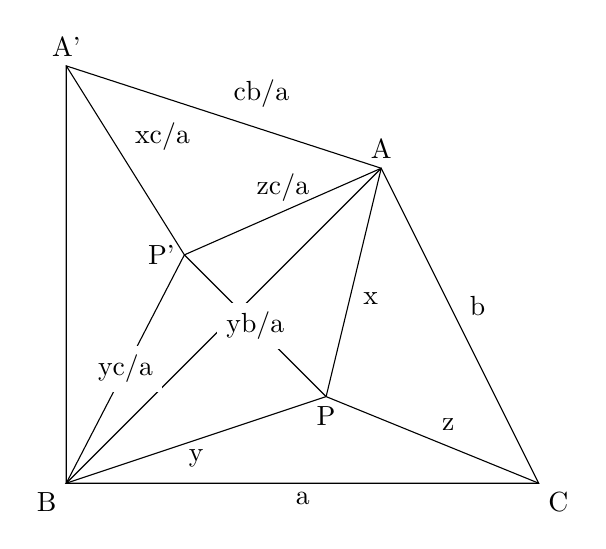
\begin{tikzpicture}
    \coordinate (A) at (1,4);
    \coordinate (B) at (-3,0);
    \coordinate (C) at (3,0);
    \coordinate (P) at (0.3,1.1);
    
    \coordinate (a) at (-3,5.3);
    \coordinate (p) at (-1.5,2.9);
    
    \node [anchor=south] at (A) {A};
    \node [anchor=north east] at (B) {B};
    \node [anchor=north west] at (C) {C};
    \node [anchor=north] at (P) {P};
    \node [anchor=south] at (a) {A'};
    \node [anchor=east] at (p) {P'};
    
    \draw (A) -- (B) -- node[anchor=north]{a} (C) -- node[anchor=south west]{b} cycle;
    \draw (P) -- node[anchor=north west]{x} (A);
    \draw (P) -- node[anchor=north]{y} (B);
    \draw (P) -- node[anchor=south west]{z} (C);
    
    \draw (B) -- (a) -- node[anchor=south west]{cb/a} (A);
    \draw (p) -- node[anchor=south]{zc/a} (A);
    \draw (p) -- node[midway , fill=white]{yc/a} (B);
    \draw (p) -- node[midway , fill=white]{yb/a} (P);
    \draw (p) -- node[anchor=south west]{xc/a} (a);
\end{tikzpicture}
\end{center}

Two things to note here are that $P'BP \sim ABC$ (by SAS) and therefore $P'AP$ is similar to the pedal triangle (by SSS). Obviously $P'BA \sim PBC$ too. The main takeaway is

`\begin{align}
    [P'BP] + [P'AP] &= [P'BA] + [PBA] \\\nonumber\\
    \frac{y^2}{a^2}[ABC] + \frac{\Delta_0}{\sin^2 A} &= \frac{c^2}{a^2}[PBC] + [PAB]
\end{align}
We use the notation $\Delta_a = [PBC], \Delta_b = [PAC], \Delta_c = [PAB]$ and we simplify this equation: (This is from rotation around $B$, two similar equations therefore arise from rotation around $A$ and $C$)
\begin{align}
    y^2\Delta + 4R^2\Delta_0 &= c^2\Delta_a + a^2\Delta_c \label{eq2} \\
    x^2\Delta + 4R^2\Delta_0 &= b^2\Delta_c + c^2\Delta_b \label{eq1} \\
    z^2\Delta + 4R^2\Delta_0 &= a^2\Delta_b + b^2\Delta_a \label{eq3} \\
    \Delta_a + \Delta_b + \Delta_c &= \Delta \label{sum}
\end{align}

The plan is to eliminate the three variables $\Delta_a, \Delta_b, \Delta_c$ from these 4 equations but before that, it must be established that \eqref{eq1}, \eqref{eq2}, \eqref{eq3}, \eqref{sum} are written assuming $P$ is inside the triangle $ABC$. In the case when $P$ is outside $ABC$ and even outside the circumcircle of $ABC$ some of these areas are to be subtracted instead of being added.

Say $P$ is outside triangle $ABC$ opposite to vertex $C$ (or across side $AB$). Then \eqref{sum} will need to replace $\Delta_c$ by $-\Delta_c$. Also, if you draw a representative figure it will be clear that \eqref{eq1} and \eqref{eq2} will also need to replace $\Delta_c$ by $-\Delta_c$. Since we plan to eliminate this variable it doesn't matter if we replace every instance of it with its negative. So we don't need to worry about $P$ crossing the triangle boundary (as such)

Say $P$ is on the circumcircle of $ABC$. Then after chasing some angles it should be clear that (say) $P',P,A$ lie on a straight line. This should help arguing the fact that as $P$ crosses the circumcircle we need to replace all instances of $\Delta_0$ with $-\Delta_0$. This would be consistent with the theorem statement. So, we can now safely proceed with equations \eqref{eq1}, \eqref{eq2}, \eqref{eq3}, \eqref{sum}. Solving for $\Delta_a$ from first three,

\begin{align}
    \Delta_a &= \Delta \left(\frac{b^2y^2 + c^2z^2 - a^2x^2}{2b^2c^2}\right) + 4R^2\Delta_0\left(\frac{b^2+c^2-a^2}{2b^2c^2}\right)
\end{align}

Also we have $\frac{b^2+c^2-a^2}{2b^2c^2} = \frac{\sin 2A}{4\Delta}$ etc. Using this we can sum up and get:
\begin{align}
    \Delta &= \Delta\left(\sum x^2 \frac{\sin 2A}{4\Delta}\right) + 4R^2\Delta_0\left(\sum \frac{\sin 2A}{4\Delta}\right) \\
    \Delta &= \frac{1}{4}\sum x^2\sin 2A + 2\Delta_0
\end{align}

This is exactly what we needed, as we already justified the change of sign for $\Delta_0$.
Q.E.D boii

\end{document}